The NI 5761 Analog Input module currently acquires data for the experiment in the following manner:
\begin{equation}\label{eq:ni_memory}
    4 \text{ channels} \cdot 250 \text{ MHz} \cdot 2 \text{ bytes/Sample} \cdot 10\ \mu\text{s/loop} \cdot 100 \text{ loops} = 2 \text{ MB .}
\end{equation}
This is to say that for the module, having 4 analog input channels, where each channel samples data at a rate of 250 MHz, with each data sample having a size of 2 bytes, collects data over a period of 10 $\mu$s. This data acquisition process is repeated 100 times per experiment cycle, all over the course of 100 ms. As a result, an amount of 2 MB of data must be stored at a time to be read and processed later for each experiment cycle. Moreover, the experiment cycle is repeated every 130 ms.

\begin{figure}[ht]
    \centering
    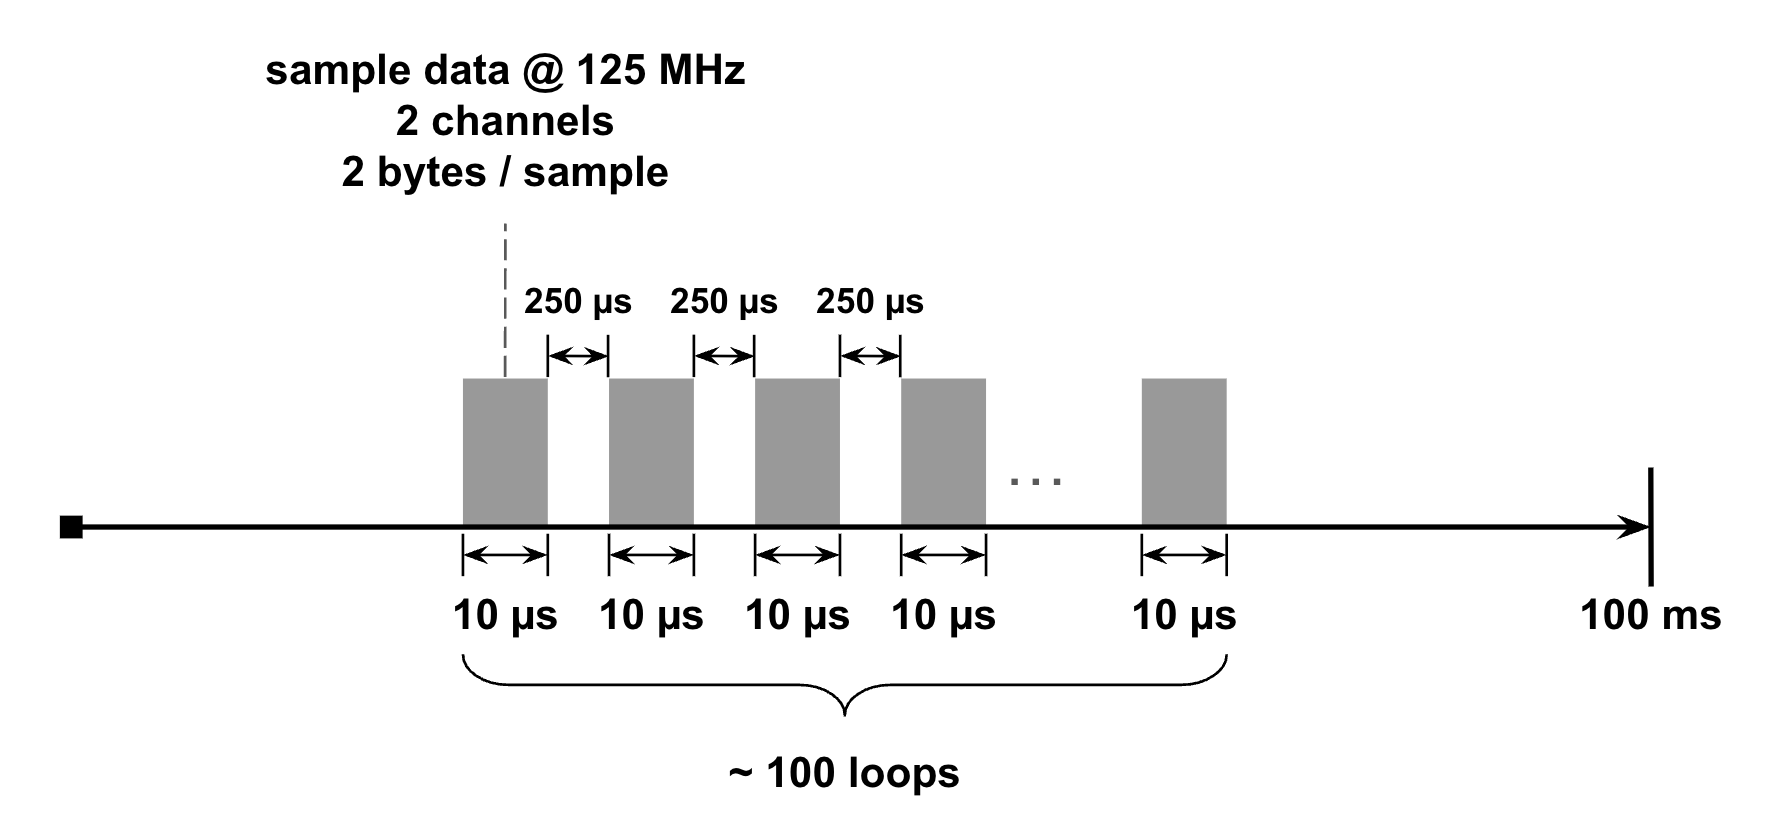
\includegraphics[width=0.85\columnwidth]{images/chapter_2/acquisition.png}
    \caption{Example schematic of how data acquisition would take place for an experimental run using the Red Pitaya, which samples data at a maximum rate of 125 million samples per second.}
    \label{fig:ch2_acquisition}
\end{figure}

Applying this acquisition process to the Red Pitaya, where there are 2 input channels and the maximum sampling rate is 125 MHz, we have
\begin{equation}\label{eq:rp_memory}
    2 \text{ channels} \cdot 125 \text{ MHz} \cdot 2 \text{ bytes/Sample} \cdot 10\ \mu\text{s/loop} \cdot 100 \text{ loops} = 0.5 \text{ MB .}
\end{equation}
This result implies that we need to be able to configure the Red Pitaya such that it can acquire and store at least 0.5 MB of input data at a given time into the on-board RAM, which has a size of 512 MB. 

In order to achieve such required memory capacity, there's a very likely need to manually extend the allocated memory space that stores the converted input signal data on the Red Pitaya for the standard oscilloscope application. So I began analyzing the Lock-in PID with Oscilloscope application, which proved rather impractical, followed by another unsuccessful attempt with the built-in Streaming service application. Finally, the Deep Memory Acquisition (DMA) feature available only in ecosystem 2.03 or newer seemed to be the most promising input acquisition method in our endeavor to use the Red Pitaya as an alternative to the NI 5761 module.

%%%%%%%%%%%%%%%%%%%%%%%%%%%%%%%%%%%%%%%%%%%%%%%%%%%%%%%%%%%%%%%%%%%%%%%%%%%%%%%%
\subsubsection{Lock-in+PID}
\subfile{../subsubsections/2_3_1_1_li_pid}

%%%%%%%%%%%%%%%%%%%%%%%%%%%%%%%%%%%%%%%%%%%%%%%%%%%%%%%%%%%%%%%%%%%%%%%%%%%%%%%%
\subsubsection{Data Streaming}
\subfile{../subsubsections/2_3_1_2_streaming}

%%%%%%%%%%%%%%%%%%%%%%%%%%%%%%%%%%%%%%%%%%%%%%%%%%%%%%%%%%%%%%%%%%%%%%%%%%%%%%%%
\subsubsection{Deep Memory Acquisition (DMA)}
\subfile{../subsubsections/2_3_1_3_dma}